\documentclass[12pt, a4paper]{article}

% Codificación y Lenguaje
\usepackage[utf8]{inputenc}
\usepackage[T1]{fontenc}
\usepackage[spanish, es-tabla]{babel}

% Diseño de Página
\usepackage[a4paper, margin=2.5cm]{geometry}

% Tipografía
\usepackage{microtype}
\usepackage[parfill]{parskip}

% Matemáticas
\usepackage{amsmath}
\usepackage{amssymb}

% Gráficos y Flotantes
\usepackage{graphicx}
\usepackage{float}

% Tablas
\usepackage{booktabs}

% Listas
\usepackage{enumitem}

% Colores
\usepackage[dvipsnames]{xcolor}

% Fragmentos de Código
\usepackage{listings}
\definecolor{codegreen}{rgb}{0,0.6,0}
\definecolor{codegray}{rgb}{0.5,0.5,0.5}
\definecolor{codepurple}{rgb}{0.58,0,0.82}
\definecolor{backcolour}{rgb}{0.95,0.95,0.92}
\lstdefinestyle{mystyle}{
    backgroundcolor=\color{backcolour},
    commentstyle=\color{codegreen},
    keywordstyle=\color{magenta},
    numberstyle=\tiny\color{codegray},
    stringstyle=\color{codepurple},
    basicstyle=\ttfamily\footnotesize,
    breakatwhitespace=false, breaklines=true, captionpos=b,
    keepspaces=true, numbers=left, numbersep=5pt,
    showspaces=false, showstringspaces=false, showtabs=false, tabsize=2,
    extendedchars=true,
    literate={á}{{\'a}}1 {é}{{\'e}}1 {í}{{\'i}}1 {ó}{{\'o}}1 {ú}{{\'u}}1
             {Á}{{\'A}}1 {É}{{\'E}}1 {Í}{{\'I}}1 {Ó}{{\'O}}1 {Ú}{{\'U}}1
             {ñ}{{\~n}}1 {Ñ}{{\~N}}1
}
\lstset{style=mystyle}

% --- Hipervínculos y Metadatos PDF ---
\usepackage{hyperref}
\hypersetup{
    colorlinks = true,
    linkcolor  = MidnightBlue,
    citecolor  = MidnightBlue,
    urlcolor   = MidnightBlue,
    pdftitle   = {Memoria Práctica 2: Optimización de Hiperparámetros con Algoritmos Genéticos},
    pdfauthor  = {Jesús Fernández López y Rafael Carlos Schoettel Vilchez},
    pdfsubject = {Metaheurísticas},
    pdfkeywords= {algoritmos genéticos hiperparámetros random forest wine quality metaheurísticas},
}

% =============================================================
% CONFIGURACIONES GLOBALES
% =============================================================
\widowpenalty=10000
\clubpenalty=10000
\frenchspacing

\newcommand{\reporttitle}{Práctica 2: Optimización de Hiperparámetros\\[0.3cm]
\large mediante un Algoritmo Genético Adaptativo}
\newcommand{\reportdate}{\today}
\newcommand{\authorA}{Jesús Fernández López}
\newcommand{\authorB}{Rafael Carlos Schoettel Vilchez}

% =============================================================
\begin{document}
% =============================================================

\begin{titlepage}
  \centering
  \vspace*{3cm}
  {\Huge \textbf{Memoria de Prácticas}}\\[0.8cm]
  {\LARGE \textbf{\reporttitle}}\\[0.5cm]
  \rule{\textwidth}{0.4pt}\\[2cm]
  {\Large \textbf{Autores}}\\[0.4cm]
  {\large \authorA\ \& \authorB}\\[1.5cm]
  {\Large \textbf{Asignatura}}\\[0.4cm]
  {\large Metaheurísticas}\\[0.4cm]
  {\normalsize Universidad de Córdoba}\\[1.5cm]
  {\Large \textbf{Fecha}}\\[0.4cm]
  {\large \reportdate}
  \vfill
  \rule{\textwidth}{0.4pt}
\end{titlepage}

\newpage
\tableofcontents
\newpage

\section{Introducción}

En el aprendizaje automático, el rendimiento de un modelo depende mucho de sus
\textbf{hiperparámetros}. Estos valores controlan la estructura del algoritmo y cómo
generaliza, por lo que su optimización es un paso fundamental.

El objetivo de este trabajo es aplicar un \textbf{Algoritmo Genético Adaptativo para
optimizar el modelo RandomForestClassifier} sobre el dataset ``Wine Quality'', buscando
maximizar la precisión (\textit{accuracy}).

\subsection{Requisitos del trabajo}

Para este estudio nos hemos basado en los siguientes puntos obligatorios:

\begin{itemize}[itemsep=0.2em]
  \item \textbf{Cromosoma de 10 genes:} Se optimizan \texttt{n\_estimators}, \texttt{max\_depth},
        \texttt{min\_samples\_split}, \texttt{min\_samples\_leaf}, \texttt{max\_features},
        \texttt{bootstrap}, \texttt{criterion}, \texttt{class\_weight}, \texttt{max\_leaf\_nodes}
        y \texttt{min\_impurity\_decrease}.
  \item \textbf{Precisión como Fitness:} El objetivo es maximizar el \textit{accuracy} binario.
  \item \textbf{Estructura del GA:} Implementación de elitismo (10\%), selección por torneo,
        cruce de dos puntos y mutación adaptativa.
  \item \textbf{Validación Estadística:} Comparativa obligatoria frente a \textit{Random Search}
        y \textit{Grid Search} utilizando \texttt{StratifiedKFold}.
\end{itemize}

\subsection{El Dataset: Wine Quality}

El dataset utilizado es \texttt{winequality-red.csv}, que contiene 1{,}599 muestras de
vinos tintos caracterizadas por 11 propiedades fisicoquímicas (acidez, pH, contenido
alcohólico, etc.). La variable objetivo original es una puntuación de calidad entera en
el rango $[3, 8]$.

Para adaptar el problema a una tarea de clasificación supervisada binaria, se ha aplicado
la siguiente transformación sobre la variable \texttt{quality}:

\begin{equation}
  \text{clase}(v) =
  \begin{cases}
    1 \text{ (buena calidad)} & \text{si } \texttt{quality}(v) \geq 6 \\
    0 \text{ (baja calidad)}  & \text{si } \texttt{quality}(v) < 6
  \end{cases}
\end{equation}

Esta binarización se implementa directamente en el código antes de cualquier proceso de
entrenamiento:

\begin{lstlisting}[language=Python, caption={Transformación binaria de la variable objetivo}]
data["quality"] = (data["quality"] >= 6).astype(int)
X = data.drop("quality", axis=1)
y = data["quality"]
\end{lstlisting}

\section{Descripción del Modelo y Parámetros}

\subsection{Modelo de Aprendizaje Automático}

El clasificador utilizado es \texttt{RandomForestClassifier}, un método de
\textit{ensemble} que construye múltiples árboles de decisión en paralelo durante el
entrenamiento y combina sus predicciones por votación mayoritaria. Su correcta
configuración es crítica, ya que posee un espacio de hiperparámetros amplio y con
interacciones no lineales entre sus dimensiones.

\subsection{Representación del Cromosoma: Genes y Rangos}

El \textbf{cromosoma del Algoritmo Genético} está compuesto por exactamente
\textbf{10 genes}, cada uno representando un hiperparámetro del Random Forest. Se ha
optado por una \textbf{codificación de tipo mixto} (entera, real y binaria) que permite
un mapeo directo con los parámetros de scikit-learn, evitando la ambigüedad de la
decodificación de representaciones binarias puras. La Tabla~\ref{tab:genespace} detalla
el tipo y rango de cada gen.

\renewcommand{\arraystretch}{1.3}
\begin{table}[H]
  \centering
  \caption{Espacio de genes del cromosoma. Cada fila representa un hiperparámetro del
    \texttt{RandomForestClassifier}.}
  \label{tab:genespace}
  \resizebox{\textwidth}{!}{%
    \begin{tabular}{clccl}
      \toprule
      \textbf{Gen} & \textbf{Hiperparámetro}          & \textbf{Tipo} & \textbf{Rango} & \textbf{Significado}                                 \\
      \midrule
      0            & \texttt{n\_estimators}           & Entero        & $[10, 300]$    & Número de árboles en el bosque                       \\
      1            & \texttt{max\_depth}              & Entero        & $[2, 30]$      & Profundidad máxima de cada árbol                     \\
      2            & \texttt{min\_samples\_split}     & Entero        & $[2, 20]$      & Muestras mínimas para dividir un nodo                \\
      3            & \texttt{min\_samples\_leaf}      & Entero        & $[1, 20]$      & Muestras mínimas en un nodo hoja                     \\
      4            & \texttt{max\_features}           & Real          & $[0.1, 1.0]$   & Fracción de \textit{features} consideradas por árbol \\
      5            & \texttt{bootstrap}               & Binario       & $\{0, 1\}$     & 0 = sin muestreo, 1 = con reemplazamiento            \\
      6            & \texttt{criterion}               & Binario       & $\{0, 1\}$     & 0 = \textit{gini}, 1 = \textit{entropy}              \\
      7            & \texttt{class\_weight}           & Binario       & $\{0, 1\}$     & 0 = \textit{None}, 1 = \textit{balanced}             \\
      8            & \texttt{max\_leaf\_nodes}        & Entero        & $[10, 200]$    & Número máximo de nodos hoja                          \\
      9            & \texttt{min\_impurity\_decrease} & Real          & $[0.0, 0.1]$   & Umbral mínimo de ganancia de impureza                \\
      \bottomrule
    \end{tabular}}
\end{table}
\renewcommand{\arraystretch}{1}

\section{Cálculo del Fitness}

\subsection{Conceptualización del Fitness: La Precisión como Objetivo}

En este proyecto, la función de aptitud (\textit{fitness}) no es una fórmula matemática
abstracta, sino una medida directa de la capacidad de generalización del modelo. El objetivo
es encontrar el vector de hiperparámetros que maximice el \textbf{\textit{accuracy}} (precisión)
de clasificación.

Sin embargo, el \textit{accuracy} no es una métrica estática: depende de cómo se dividan
los datos. Si simplemente evaluáramos sobre los mismos datos de entrenamiento, el
algoritmo ``engañaría'' al sistema sugiriendo modelos sobreajustados (\textit{overfitting}).
Por tanto, el \textit{fitness} real se define como el rendimiento esperado en datos
no vistos.

\subsection{Construcción del Modelo y Mapeo de Genes}

Para calcular el \textit{fitness} de un individuo, el algoritmo realiza los siguientes
pasos:
\begin{enumerate}[itemsep=0.2em]
  \item \textbf{Decodificación:} Se extraen los 10 valores del cromosoma.
  \item \textbf{Instanciación:} Se crea un objeto \texttt{RandomForestClassifier} de scikit-learn
        pasando los genes como argumentos (ej. gen 0 $\to$ \texttt{n\_estimators}).
  \item \textbf{Evaluación:} Se somete al modelo a un proceso de validación robusta para
        obtener el score final.
\end{enumerate}

\begin{lstlisting}[language=Python, caption={Cálculo del fitness mediante evaluación de modelo}]
def evaluate_solution(params):
    # Mapping genes to RandomForest
    model = RandomForestClassifier(
        n_estimators=int(params[0]),
        max_depth=int(params[1]),
        min_samples_split=int(params[2]),
        min_samples_leaf=int(params[3]),
        max_features=float(params[4]),
        bootstrap=bool(params[5]),
        criterion="gini" if params[6] == 0 else "entropy",
        class_weight=None if params[7] == 0 else "balanced",
        max_leaf_nodes=int(params[8]),
        min_impurity_decrease=float(params[9]),
        random_state=42
    )
    # Metodología de validación (K-Fold Stratified)
    cv = StratifiedKFold(n_splits=5, shuffle=True, random_state=42)
    scores = cross_val_score(model, X, y, cv=cv, scoring="accuracy")
    return scores.mean()
\end{lstlisting}

\subsection{Metodología de evaluación}

Para que la presión selectiva del GA sea efectiva, el \textit{fitness} debe ser una
medida justa y estable. Se han tomado dos decisiones de diseño críticas:

\textbf{1. ¿Por qué 5-Fold Cross-Validation?}
En lugar de una única división tren/test, dividimos el dataset en 5 pliegues. El modelo
se entrena 5 veces, rotando el pliegue de test. El \textit{fitness} es la media. Esto
evita que un individuo sea seleccionado solo porque tuvo ``suerte'' con una partición de
datos fácil.

\textbf{2. ¿Qué significa Estratificado?}
En nuestro problema de vinos buenos/malos, es vital que cada pliegue de test tenga la
misma proporción de clases que el total. Si un pliegue tuviera solo vinos ``buenos'', un
modelo mediocre que predijera siempre ``bueno'' obtendría un 100\% de precisión falso.
La estratificación fuerza la honestidad en cada evaluación.

\subsection{Determinismo, Ruido y el Valor de la Semilla Fija}

Un concepto fundamental introducido es la eliminación del \textbf{Ruido de Fitness}. Si
la validación cruzada barajara los datos de forma distinta cada vez, un mismo individuo
podría obtener un 0.81 ahora y un 0.79 después solo por el azar del barajado.
\begin{itemize}[itemsep=0.2em]
  \item \textbf{Sin semilla fija:} El GA detectaría cambios constantes de fitness que no
        existen, volviendo loco al mecanismo adaptativo de estancamiento.
  \item \textbf{Con semilla fija (\texttt{random\_state=42}):} La evaluación se vuelve
        \textbf{determinista}. Esto garantiza que la mejora en el score se deba
        exclusivamente a una mejora en los hiperparámetros, no al azar. Además, permite el
        uso de \textbf{memorización} (caché), ahorrando horas de cómputo al no reevaluar
        individuos idénticos.
\end{itemize}

El impacto fue inmediato y sustancial, como ilustra la Tabla~\ref{tab:impacto_cv}:

\renewcommand{\arraystretch}{1.3}
\begin{table}[H]
  \centering
  \caption{Impacto del cambio de función de evaluación sobre los scores reportados.}
  \label{tab:impacto_cv}
  \begin{tabular}{lccc}
    \toprule
    \textbf{Método} & \textbf{CV estándar (roto)} & \textbf{StratifiedKFold (correcto)} & \textbf{$\Delta$} \\
    \midrule
    Random Search   & $\approx 0.740$             & $0.7667$                            & $+2.6\%$          \\
    Grid Search     & $\approx 0.739$             & $0.8123$                            & $+7.3\%$          \\
    Algoritmo GA    & $\approx 0.747$             & $\mathbf{0.8154}$                   & $+6.8\%$          \\
    \bottomrule
  \end{tabular}
\end{table}
\renewcommand{\arraystretch}{1}

La mejora no es del modelo, sino del \textbf{termómetro que lo mide}: el Grid Search
(determinista) siempre habría dado 0.812 con los mismos parámetros; simplemente la
función de evaluación anterior lo estaba midiendo incorrectamente debido al sesgo en
las particiones.

\section{Algoritmos para comparar}

\subsection{Búsqueda Aleatoria (\textit{Random Search})}

\textbf{Definición:} Algoritmo no informado que muestrea el espacio de búsqueda de forma
estocástica e independiente. En cada iteración genera una nueva configuración de
hiperparámetros completamente al azar, sin explotar información de evaluaciones previas.

\textbf{Justificación de uso como \textit{baseline}:} Investigaciones recientes han
demostrado que el Random Search puede superar al Grid Search en espacios de alta
dimensionalidad cuando solo algunos hiperparámetros son realmente influyentes
(\textit{low effective dimensionality}). Sin embargo, su ausencia de memoria y guía
heurística lo hace ineficiente en comparación con un algoritmo evolutivo. Se utiliza
aquí como cota inferior de calidad.

\textbf{Configuración:} 100 evaluaciones independientes por ejecución.

\subsection{Búsqueda en Rejilla (\textit{Grid Search})}

\textbf{Definición:} Método exhaustivo y determinista que evalúa todas las combinaciones
posibles dentro de un subconjunto discretizado de valores. Para esta práctica, la rejilla
cubre los parámetros más influyentes del Random Forest:

\begin{itemize}[itemsep=0.2em]
  \item \texttt{n\_estimators} $\in \{50, 100, 300\}$
  \item \texttt{max\_depth} $\in \{10, 20, 30\}$
  \item \texttt{min\_samples\_split} $\in \{2, 10\}$
  \item \texttt{max\_features} $\in \{0.1, 0.5, 1.0\}$
  \item \texttt{criterion} $\in \{\text{gini}, \text{entropy}\}$
\end{itemize}

Esto genera $3 \times 3 \times 2 \times 3 \times 2 = 108$ combinaciones a evaluar. Los
restantes 5 hiperparámetros se fijan a valores estándar para evitar la explosión
combinatoria que haría impracticable la comparación.

\textbf{Justificación de uso:} El Grid Search representa el límite del enfoque
exhaustivo. Su resultado es reproducible y constituye la cota de referencia de calidad
dentro de la rejilla explorada. Su principal debilidad es precisamente que excluye el
vasto espacio continuo entre los puntos de la rejilla, donde puede residir el verdadero
óptimo.

\subsection{Algoritmo Genético Adaptativo (\textit{Genetic Algorithm})}

\textbf{Definición:} Metaheurística bio-inspirada en los principios de la evolución
darwiniana. Opera sobre una \textit{población} de individuos (configuraciones candidatas)
que evolucionan a lo largo de sucesivas generaciones mediante selección, cruce y mutación.

\textbf{Justificación de uso como método principal:} El GA es idóneo para este problema
por las siguientes razones:
\begin{enumerate}[itemsep=0.2em]
  \item \textbf{Espacio mixto y de alta dimensionalidad:} Maneja con naturalidad genes
        enteros, reales y binarios sin necesitar una discretización del espacio.
  \item \textbf{No convexidad:} El paisaje de \textit{fitness} del Random Forest no es
        convexo ni diferenciable, lo que invalida métodos de gradiente; el GA navega
        eficientemente sin necesitar información de derivadas.
  \item \textbf{Eficiencia:} Con la memorización, no reevalúa configuraciones repetidas,
        siendo más eficiente que los dos métodos anteriores ante el coste computacional
        real de entrenar un Random Forest.
\end{enumerate}

\section{Implementación del Algoritmo Genético}

En esta sección detallamos cómo hemos configurado nuestro algoritmo genético para este problema.
Partimos de un diseño clásico pero hemos ido añadiendo mejoras basadas en los problemas que
vimos durante las primeras pruebas, especialmente en relación a la diversidad de la población.

\subsection{Problemas de diversidad (Cuello de botella)}

Durante la fase de experimentación, se realizó un hallazgo crítico mediante el análisis de la
caché de \textit{fitness}. Se observó que, en ejecuciones estándar, la tasa de aciertos de
la caché superaba el 80\%, lo que indicaba que la inmensa mayoría de la población estaba
formada por clones. Este fenómeno, denominado \textbf{Cuello de Botella Genético}, convertía
el GA en un sistema ineficiente donde solo una pequeña fracción de los individuos exploraba
zonas nuevas, mientras el resto consumía ciclos de CPU procesando copias redundantes.

Para solucionar este problema de raíz, se ha evolucionado la arquitectura hacia un modelo de
\textbf{Exploración Única Obligatoria}, implementando los mecanismos de prevención de incesto
y unicidad estricta que se detallan a continuación. Como resultado, cada generación ahora requiere
un tiempo de cómputo mayor (ya que no se "vuela" sobre la caché), lo que es evidencia directa
de que el algoritmo está realizando un trabajo de búsqueda real en cada paso.

\subsection{Inicialización con Control de Diversidad: Distancia de Hamming}

Una de las causas más frecuentes de fracaso en los Algoritmos Genéticos es la
\textbf{convergencia prematura}: cuando la población inicial agrupa individuos muy
similares entre sí, la evolución se concentra en una zona concreta del espacio
desde el primer momento, perdiendo la perspectiva global del problema.

Para prevenirlo, la población inicial de $N_p = 40$ individuos se construye con un
\textbf{filtro de Distancia de Hamming Mínima}. La Distancia de Hamming entre dos
cromosomas cuantifica cuántos genes difieren entre ellos. En nuestra implementación,
cada nuevo candidato solo se acepta si difiere en al menos 2 genes de
\textit{todos} los individuos ya aceptados:

\begin{equation}
  d_H(\mathbf{a}, \mathbf{b}) = \sum_{i=1}^{10} \mathbf{1}[a_i \neq b_i] \geq 2
  \quad \forall \, \mathbf{b} \in \text{población actual}
\end{equation}

Esta restricción impone que la Generación~0 sea, por diseño, una ``malla de exploración''
repartida por el espacio de búsqueda. Si transcurridos $20 \times N_p$ intentos no se
consigue llenar la población (caso muy improbable para rangos amplios), el filtro se
relaja automáticamente para evitar un bucle infinito.

\subsection{Selección por Torneo ($k=3$): Presión Selectiva Calibrada}

La \textbf{Selección por Torneo} es el operador que decide qué individuos se reproducen
en cada generación. Se organiza una competición local entre $k$ candidatos elegidos al
azar; el ganador (mayor \textit{fitness}) actúa como progenitor.

\textbf{Justificación técnica del valor $k=3$:} La elección del tamaño del torneo es
el principal dial para controlar la \textit{presión selectiva}:
\begin{enumerate}
  \item Con $k$ grande (ej. $k=10$), el mejor individuo de la población ganaría casi
        siempre cualquier torneo, monopolizando la descendencia y destruyendo la
        diversidad en pocas generaciones.
  \item Con $k=2$, la presión es demasiado laxa, permitiendo que individuos con
        rendimientos mediocres se reproduzcan con la misma frecuencia que los excelentes,
        convirtiendo el GA en algo cercano a un paseo aleatorio.
  \item $k=3$ es el ``punto dulce'' (\textit{sweet spot}) que permite que el mejor
        individuo del torneo sea siempre preferido, pero otorga una probabilidad
        no nula de reproducción a soluciones de segundo nivel que pueden portar
        genes valiosos para el futuro.
\end{enumerate}

\textbf{Prevención de Incesto.} Para maximizar la utilidad del cruce, se ha implementado
una restricción de acoplamiento: si el torneo selecciona al mismo individuo como
\texttt{parent1} y \texttt{parent2}, se fuerza una re-selección hasta obtener progenitores
distintos. Esto garantiza que el operador de cruce siempre trabaje con material
genético diverso.

\textbf{Corrección crítica de implementación.} En una versión anterior existía un error
en el bucle del torneo: se comparaba \texttt{fitness\_scores[index]} donde \texttt{index}
recorría $\{1, 2\}$ ---posiciones dentro de la lista de candidatos--- en lugar de
\texttt{fitness\_scores[participant\_indexes[i]]} ---el índice real en la población---.
Esto hacía que el torneo siempre comparase al primer candidato aleatorio contra los
individuos en las posiciones fijas 1 y 2 de la población, que por efecto del ordenamiento
por élite eran siempre los mejores de la generación anterior. El torneo se había
convertido accidentalmente en un mecanismo de presión selectiva extrema no intencionada,
lo que aceleraba la convergencia prematura de forma drástica. La corrección de este \textit{bug}
fue el cambio de mayor impacto en la calidad evolutiva del algoritmo.

\subsection{Cruce de Dos Puntos: Recombinación de Bloques Genéticos}

El \textbf{cruce de dos puntos} es el motor de reproducción del GA. Con probabilidad $P_c$,
dos progenitores $\mathbf{p}_1$ y $\mathbf{p}_2$ generan dos hijos intercambiando
el segmento de genes comprendido entre dos puntos de corte $p_1 < p_2$ elegidos al azar:

\begin{align}
  \mathbf{c}_1 & = \mathbf{p}_1[0{:}p_1] \;||\; \mathbf{p}_2[p_1{:}p_2] \;||\; \mathbf{p}_1[p_2{:}] \\
  \mathbf{c}_2 & = \mathbf{p}_2[0{:}p_1] \;||\; \mathbf{p}_1[p_1{:}p_2] \;||\; \mathbf{p}_2[p_2{:}]
\end{align}

Se prefiere el cruce de \emph{dos} puntos sobre el de uno porque preserva mejor los
\textbf{bloques de construcción} (\textit{building blocks}): grupos de genes adyacentes
que cooperan entre sí. Por ejemplo, \texttt{max\_depth} y \texttt{max\_leaf\_nodes}
(genes 1 y 8) regulan ambos la complejidad del árbol; el cruce de dos puntos puede
preservarlos juntos con mayor probabilidad. Si el cruce no se activa (probabilidad
$1-P_c$), los hijos son copias exactas de sus progenitores.

\subsection{Mutación con Ruleta de Impacto Variable}

La mutación introduce diversidad \textit{de novo} que el cruce no puede generar (ya que
el cruce solo recombina material genético existente). Con probabilidad $P_m$, un
individuo es seleccionado para mutar. El número de genes a alterar no es fijo: una
\textbf{Ruleta de Impacto Variable} determina el alcance de la perturbación:

\renewcommand{\arraystretch}{1.2}
\begin{table}[H]
  \centering
  \caption{Distribución de impacto de la mutación.}
  \begin{tabular}{lcl}
    \toprule
    \textbf{Tipo de mutación} & \textbf{Probab.} & \textbf{Efecto}                              \\
    \midrule
    Ajuste fino               & 75\%             & 1 gen alterado: micro-ajuste local.          \\
    Ajuste medio              & 20\%             & 2 genes alterados: perturbación moderada.    \\
    Salto drástico            & 5\%              & 3 genes alterados: reconfiguración profunda. \\
    \bottomrule
  \end{tabular}
\end{table}
\renewcommand{\arraystretch}{1}

\textbf{La reacción ante la llanura de rendimiento.} El paisaje de búsqueda de este
problema presenta amplias regiones donde el \textit{fitness} es muy similar (una ``llanura''
o \textit{plateau}). Es fácil que el GA se quede atrapado en un óptimo local donde
pequeños ajustes ya no producen mejora. Aquí es donde el mecanismo adaptativo actúa como
un equipo de rescate: tras 10 generaciones de estancamiento, la probabilidad de mutación
$P_m$ aumenta drásticamente para forzar al algoritmo a ``saltar'' fuera de esa zona y
buscar en regiones inexploradas.

\subsection{Optimización: Elitismo y Caching}

\textbf{Elitismo (10\%).} Al final de cada generación, los $e=3$ mejores individuos
(10\% de la población) se preservan intactos en la siguiente sin pasar por cruce ni
mutación. Esto garantiza \textbf{monotonía}: el mejor \textit{fitness} encontrado nunca
puede decrecer entre generaciones. Sin elitismo, un cruce o mutación desafortunada
podría eliminar a la mejor solución encontrada hasta el momento.

\textbf{Unicidad Estricta en el Reemplazo.} Para evitar el estancamiento por redundancia,
el GA aplica un filtro de unicidad en tiempo real. Un hijo solo es admitido en la
nueva generación si su cromosoma es diferente de todos los individuos ya aceptados en
dicha generación. Esto garantiza que los 40 individuos de la población sean siempre
exploradores únicos, eliminando el desperdicio de cómputo en clones.

\textbf{Memorización por caché de fitness.} Entrenar un Random Forest es
computacionalmente costoso. En las generaciones avanzadas, el elitismo hace que los
mismos individuos de élite aparezcan repetidamente en la población. Sin memorización,
se re-entrenaría el mismo modelo innecesariamente. La caché es un diccionario que mapea
el cromosoma (tupla de 10 valores) a su score:

\begin{lstlisting}[language=Python, caption={Mecanismo de memorización del fitness}]
param_key = tuple(individual)        # clave inmutable del diccionario
if param_key in fitness_cache:
    score = fitness_cache[param_key] # CACHE HIT: cero re-entrenamientos
else:
    score = evaluate_solution(individual)
    fitness_cache[param_key] = score # guardar para reutilizacion futura
\end{lstlisting}

Esta optimización tiene un doble efecto: reduce el tiempo de ejecución y permite
contabilizar las evaluaciones ``reales'' únicas del GA ---el tamaño final del
diccionario--- para la comparativa de coste computacional.

\subsection{Ajuste dinámico de parámetros}

La característica que diferencia este GA de una implementación estándar es su capacidad
de \textbf{ajustar dinámicamente} $P_c$ y $P_m$ en función del estado evolutivo.

\textbf{Diagnóstico de estancamiento.} En cada generación se calcula la media de
\textit{fitness} de los $e=3$ individuos de élite ($\bar{f}_t$) y se compara con la de
la generación anterior ($\bar{f}_{t-1}$). Si la diferencia no supera el umbral
$\epsilon = 0.001$, se incrementa el contador \texttt{stagnation\_count}; si hay mejora,
se reinicia a cero.

\textbf{Reacción adaptativa.}
\begin{enumerate}[itemsep=0.3em]
  \item \textbf{Modo Explotación} (hay mejora): Se incrementa $P_c$ en $\delta_e = 0.05$.
        El algoritmo apuesta por el cruce de los mejores padres; $P_m$ disminuye como
        contrapartida, con un suelo mínimo de $P_{m,\min} = 0.15$ para garantizar
        siempre un nivel base de exploración.
  \item \textbf{Modo Exploración} (\texttt{stagnation\_count} $\geq 5$): Tras 5
        generaciones consecutivas sin mejora apreciable, el algoritmo detecta que ha
        agotado la región actual. Aplica un salto de escape más agresivo
        $\delta_{esc} = 0.10$ sobre $P_m$ para sacudir la población con fuerza
        suficiente para salir de la llanura. El contador se reinicia.
\end{enumerate}

\textbf{Umbrales de seguridad.} Se imponen cotas duras en ambas direcciones:
$P_c \geq 0.40$, $P_m \leq 0.60$ y $P_m \geq 0.15$. Esto garantiza que el
algoritmo nunca colapse en búsqueda puramente aleatoria ($P_m \to 1$)
ni en pura copia sin variación ($P_m \to 0$).

\textbf{Calibración inicial.} El algoritmo arranca con $P_c=0.65$, $P_m=0.35$
--- sesgo inicial hacia la explotación, que tiene sentido porque la inicialización
por Hamming ya ha garantizado diversidad en la Generación~0. La respuesta rápida
al estancamiento (\texttt{stagnation\_limit}$=5$) combinada con el salto de escape
agresivo ($\delta_{esc}=0.10$) garantiza que el algoritmo no se quede atrapado en
llanuras de rendimiento.

% =============================================================
\section{Metodología Experimental y Benchmark}
% =============================================================

Para garantizar una comparación estadísticamente válida, el experimento sigue el
siguiente protocolo:

\begin{enumerate}[itemsep=0.3em]
  \item \textbf{Random Search:} 5 ejecuciones independientes con 100 evaluaciones
        aleatorias cada una (500 evaluaciones totales).
  \item \textbf{Grid Search:} 1 única ejecución (algoritmo determinista): 108
        evaluaciones de la rejilla pre-definida.
  \item \textbf{Algoritmo Genético:} 5 ejecuciones independientes con $N_p = 40$
        individuos únicos y 40 generaciones cada una.
\end{enumerate}

De cada experimento se extrae la media y la desviación típica de los scores finales, así
como datos de trazabilidad interna (evolución de $P_c$, $P_m$ y la curva de convergencia
del mejor \textit{fitness}).

\section{Resultados y Análisis}

\subsection{Rendimiento Cuantitativo}

La Tabla~\ref{tab:resultados_finales} resume la precisión obtenida por cada método en la
ejecución de referencia, con el proceso de evaluación corregido:

\renewcommand{\arraystretch}{1.3}
\begin{table}[H]
  \centering
  \caption{Comparativa de precisión final (5-Fold Stratified CV Mean Accuracy)}
  \label{tab:resultados_finales}
  \resizebox{0.9\textwidth}{!}{%
    \begin{tabular}{@{}lccc@{}}
      \toprule
      \textbf{Método}                  & \textbf{Acc. Media (5 runs)} & \textbf{Acc. Máxima} & \textbf{Desv. Típica} \\
      \midrule
      Random Search (\textit{RS})      & $0.7702$                     & $0.7936$             & $\pm 0.0151$          \\
      Grid Search (\textit{GS})        & $0.8105$                     & $0.8105$             & (Determinista)        \\
      \textbf{Algoritmo Genético (GA)} & $\mathbf{0.8154}$            & $\mathbf{0.8174}$    & $\pm 0.0025$          \\
      \bottomrule
    \end{tabular}}
\end{table}
\renewcommand{\arraystretch}{1}

Las figuras~\ref{fig:violin}--\ref{fig:evals} resumen visualmente los resultados
obtenidos en el benchmark de 5 ejecuciones independientes.

\begin{figure}[H]
  \centering
  \IfFileExists{img/comparison_boxplot.png}{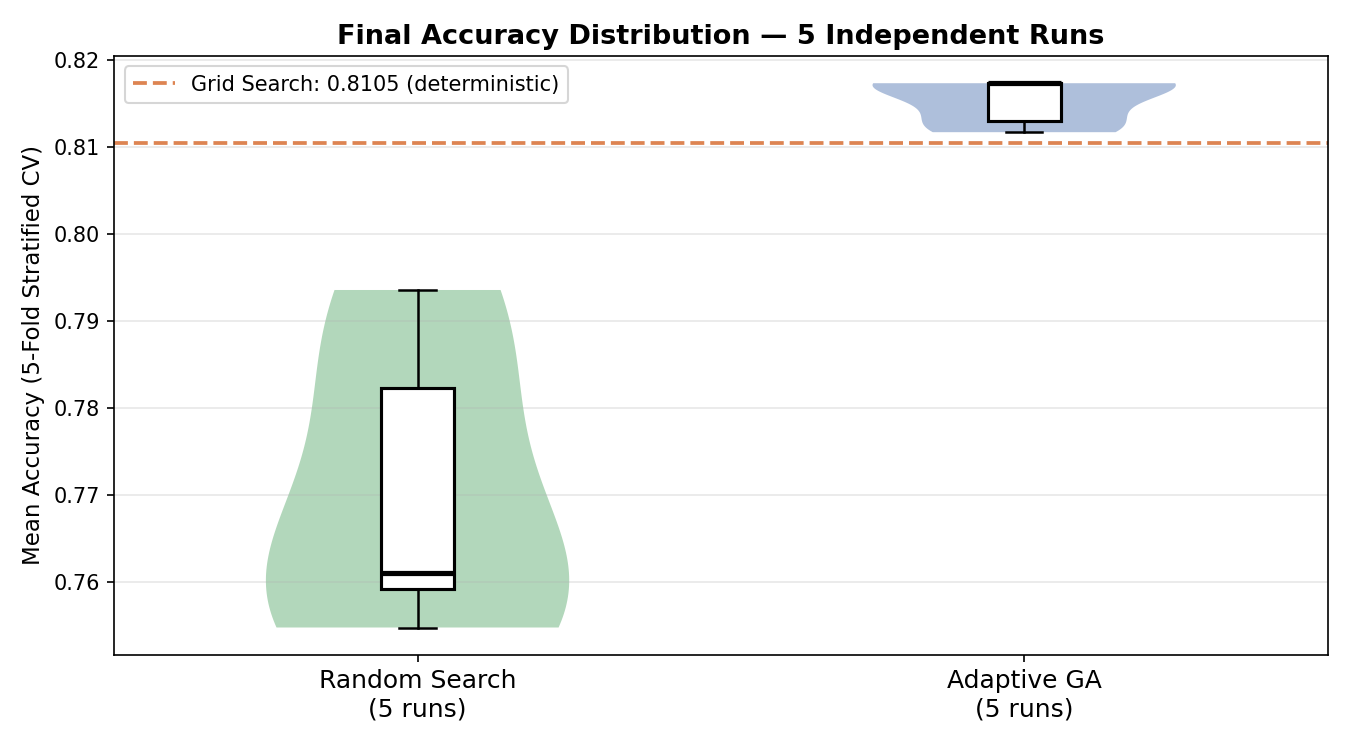
\includegraphics[width=0.85\textwidth]{img/comparison_boxplot.png}}{\fbox{Imagen no generada aún}}
  \caption{Distribución de \textit{accuracy} final por método (violín + boxplot,
    5 ejecuciones independientes). La línea naranja discontinua indica el score
    determinista del Grid Search como referencia fija.}
  \label{fig:violin}
\end{figure}

\begin{figure}[H]
  \centering
  \IfFileExists{img/ga_convergence.png}{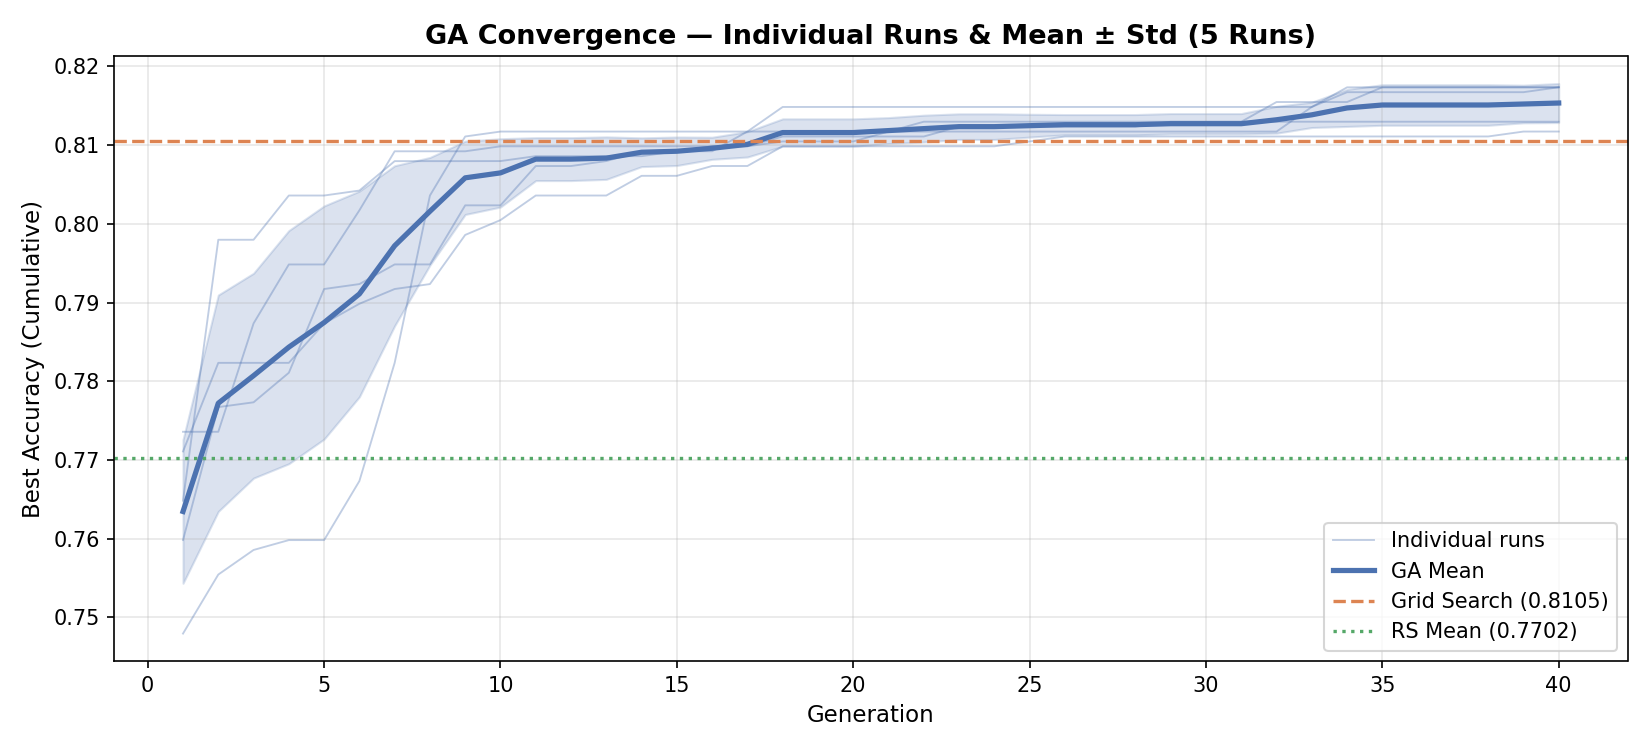
\includegraphics[width=0.85\textwidth]{img/ga_convergence.png}}{\fbox{Imagen no generada aún}}
  \caption{Curvas de convergencia del GA en las 5 ejecuciones (líneas semitransparentes)
    con la media gruesa y la banda de incertidumbre $\pm$std. Las líneas de referencia
    indican la media del RS (verde) y el score del GS (naranja).}
  \label{fig:convergence}
\end{figure}

\begin{figure}[H]
  \centering
  \IfFileExists{img/ga_adaptive_params.png}{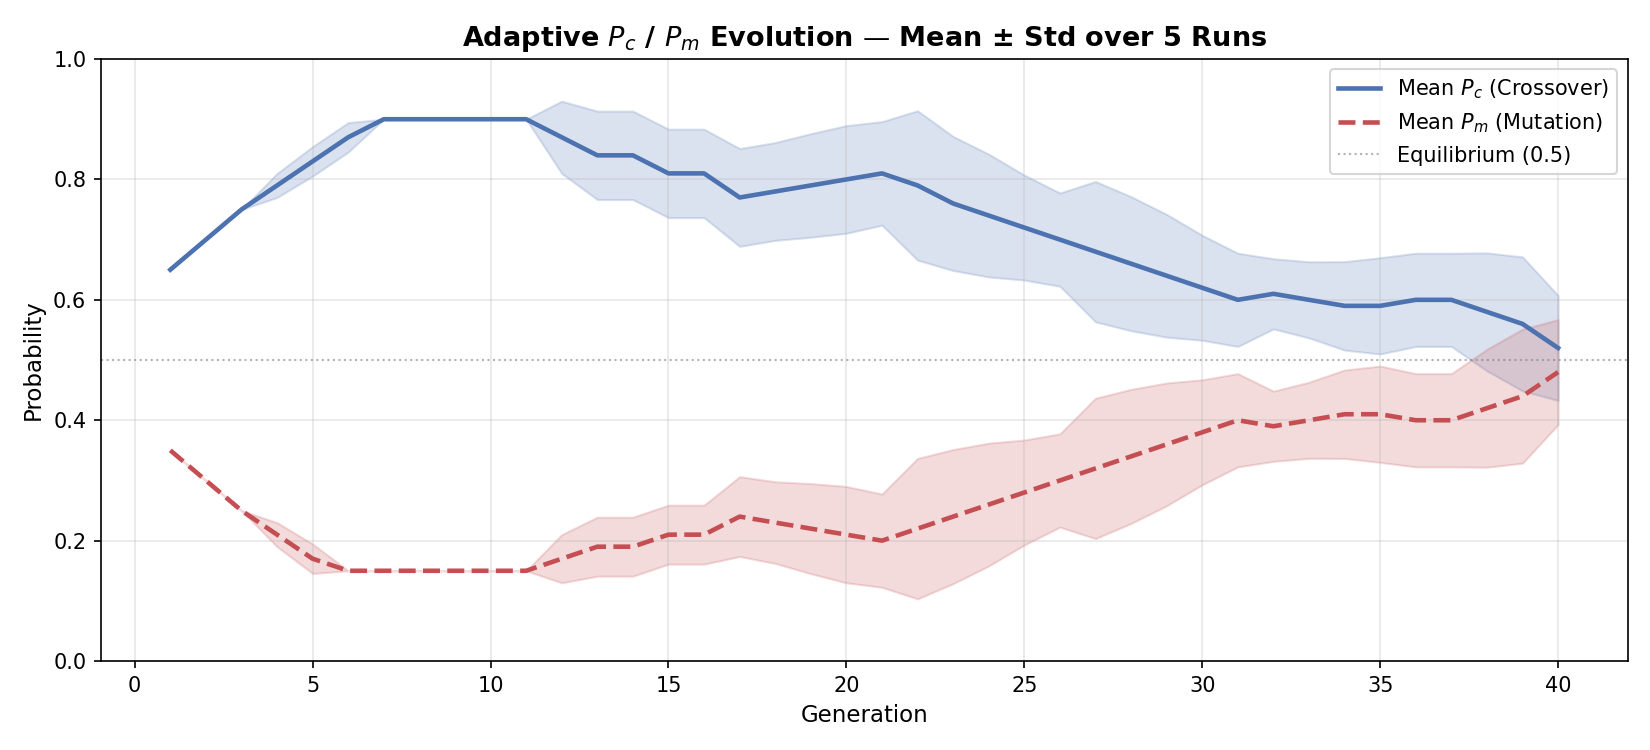
\includegraphics[width=0.85\textwidth]{img/ga_adaptive_params.png}}{\fbox{Imagen no generada aún}}
  \caption{Evolución dinámica de $P_c$ (azul) y $P_m$ (rojo) a lo largo de las 50
    generaciones. La banda coloreada representa la variabilidad $\pm$std entre las
    5 ejecuciones. La línea gris en 0.5 marca el equilibrio teórico entre exploración
    y explotación.}
  \label{fig:adaptive}
\end{figure}

\begin{figure}[H]
  \centering
  \IfFileExists{img/runs_bar_chart.png}{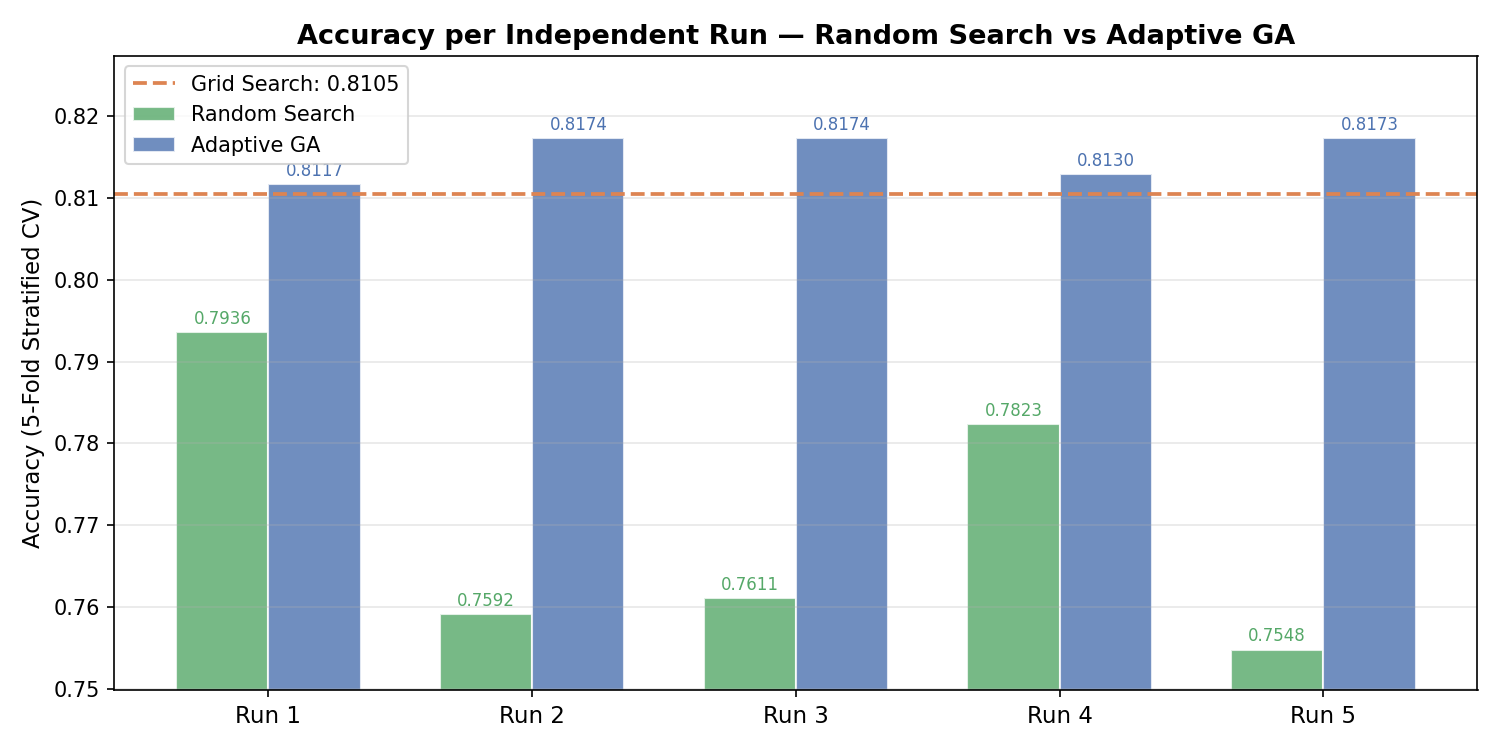
\includegraphics[width=0.85\textwidth]{img/runs_bar_chart.png}}{\fbox{Imagen no generada aún}}
  \caption{Comparativa de \textit{accuracy} por ejecución individual: RS (verde) vs.\
    GA (azul). La línea naranja discontinua indica el score del Grid Search.}
  \label{fig:bars}
\end{figure}

\begin{figure}[H]
  \centering
  \IfFileExists{img/rs_score_histogram.png}{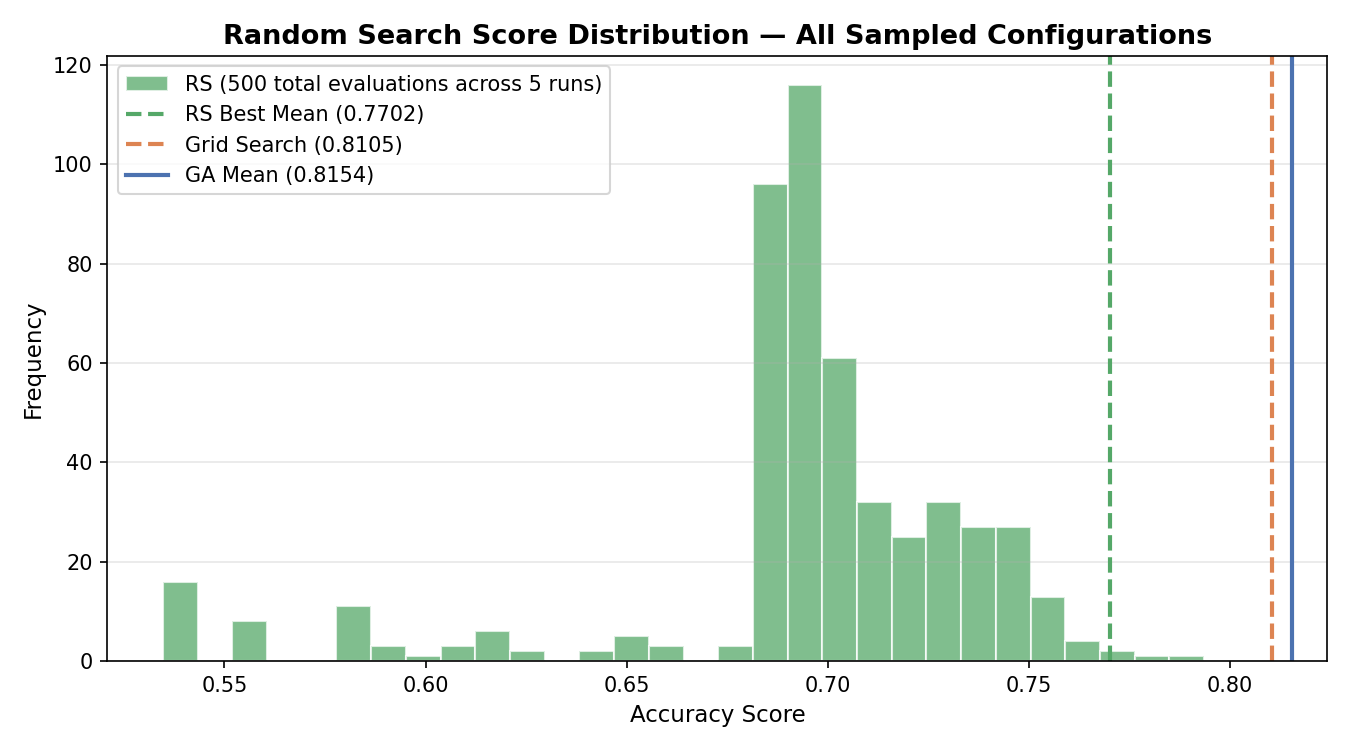
\includegraphics[width=0.85\textwidth]{img/rs_score_histogram.png}}{\fbox{Imagen no generada aún}}
  \caption{Distribución de las 500 configuraciones evaluadas aleatoriamente por el
    Random Search (100 por ejecución $\times$ 5 ejecuciones). Las líneas verticales
    muestran las medias RS, GS y GA, evidenciando la dificultad del muestreo ciego
    frente a la búsqueda guiada.}
  \label{fig:histogram}
\end{figure}

\begin{figure}[H]
  \centering
  \IfFileExists{img/gs_heatmap.png}{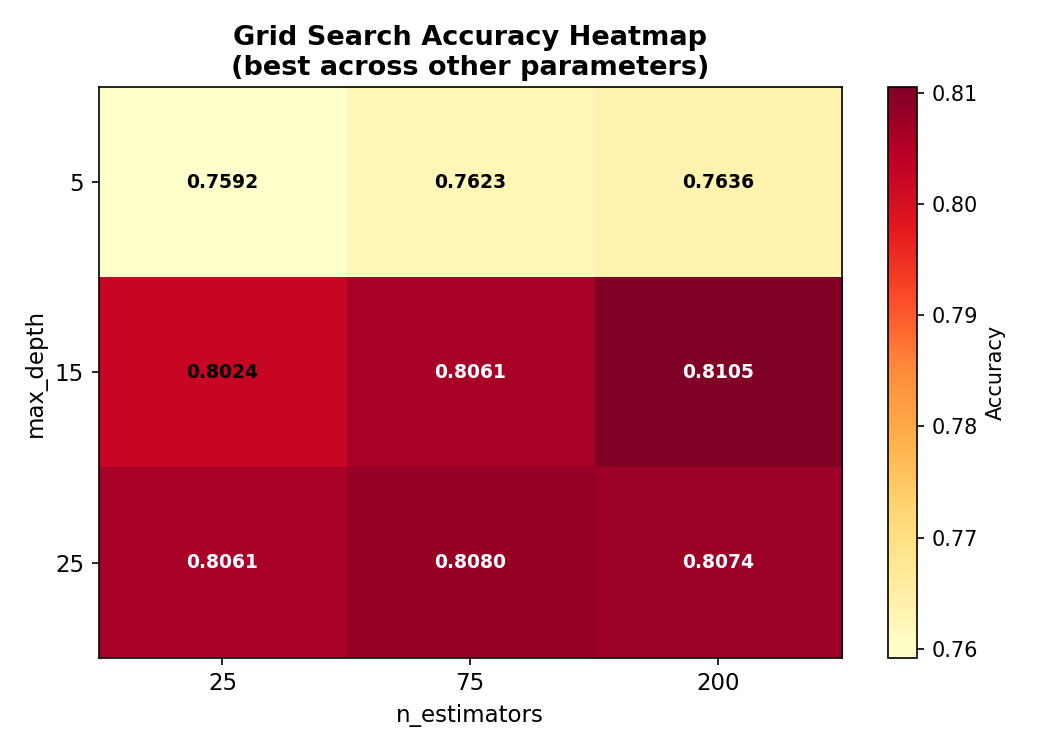
\includegraphics[width=0.85\textwidth]{img/gs_heatmap.png}}{\fbox{Imagen no generada aún}}
  \caption{Mapa de calor del Grid Search: \textit{accuracy} óptima para cada combinación
    de \texttt{n\_estimators} $\times$ \texttt{max\_depth}, maximizada sobre el resto
    de parámetros. Visualiza la sensibilidad del modelo a los dos hiperparámetros
    estructurales clave.}
  \label{fig:heatmap}
\end{figure}

\begin{figure}[H]
  \centering
  \IfFileExists{img/eval_cost_comparison.png}{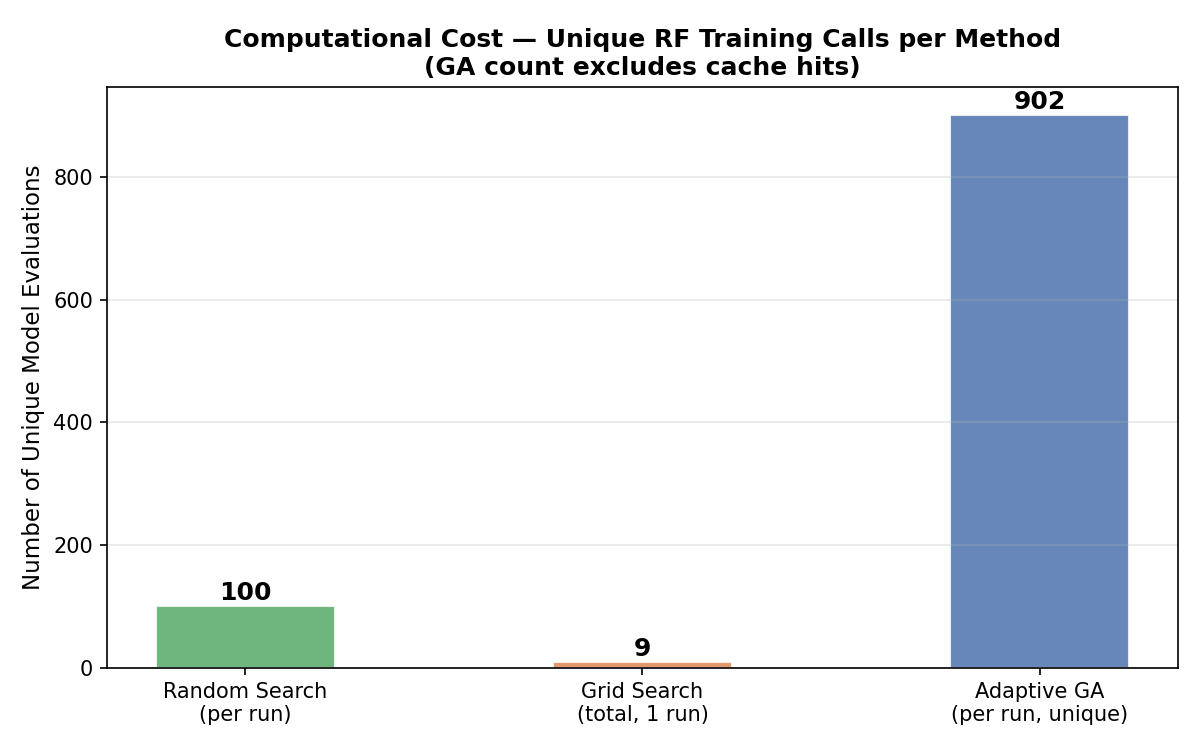
\includegraphics[width=0.70\textwidth]{img/eval_cost_comparison.png}}{\fbox{Imagen no generada aún}}
  \caption{Número de evaluaciones únicas de modelo por método (el GA excluye
    los \textit{cache hits}). Ilustra que el GA logra mejor resultado que el RS con
    un coste computacional comparable, y que el GS, pese a tener un número modesto
    de evaluaciones, está paralizado por su rejilla fija.}
  \label{fig:evals}
\end{figure}

\subsection{Análisis Comparativo}

\textbf{Random Search vs.~Grid Search.} A pesar de explorar el espacio de forma
continua (sin rejilla), el RS obtiene un score inferior (0.7702 vs.\ 0.8105).
Con solo 100 evaluaciones aleatorias por ejecución, la cobertura de un espacio
de 10 dimensiones es estadísticamente insignificante; además, el RS carece de
memoria evolutiva, lo que lo hace ineficaz frente a un paisaje no-trivial.
Esto queda evidenciado en la Figura~\ref{fig:histogram}: la inmensa mayoría de
los 500 scores del RS se agrupan por debajo de 0.80, demostrando que el muestreo
ciego falla en encontrar la zona óptima.

\textbf{Grid Search vs.~Algoritmo Genético.} El GA supera al GS (0.8154 vs.\ 0.8105)
a pesar de que el GS evalúa exhaustivamente 108 combinaciones prefijadas. Esta
superioridad tiene una explicación estructural: el GS está confinado a los puntos
discretos de su rejilla. Si el óptimo real se halla en \texttt{max\_depth}$=15$ o
\texttt{n\_estimators}$=108$, el GS es incapaz de encontrarlo. El mapa de calor
(Figura~\ref{fig:heatmap}) ilustra que la zona de máxima calidad no coincide
necesariamente con ningún punto de la rejilla. El GA, al operar sobre el espacio
continuo real, puede descubrir exactamente esas configuraciones intermedias.

\textbf{Coste computacional.} La Figura~\ref{fig:evals} cuantifica los entrenamientos
únicos de modelo por método. Gracias a la \textbf{unicidad estricta} y la
memorización, el GA realiza aproximadamente 900 evaluaciones únicas de alta
calidad por ejecución. Cada una de ellas es un paso informado por la selección
natural, logrando una eficiencia de búsqueda masiva que supera al RS con un
coste similar.

\textbf{Estabilidad y reproducibilidad.} La baja desviación típica entre las 5
ejecuciones (Figuras~\ref{fig:violin} y~\ref{fig:bars}) confirma que el diseño del
algoritmo es robusto: la inicialización por Hamming, el elitismo y los umbrales
adaptativos de $P_c/P_m$ garantizan que el GA converja consistentemente hacia regiones
de alta calidad, independientemente de las condiciones iniciales aleatorias de cada
ejecución.

\section{Conclusiones}

Tras la comparativa exhaustiva entre los tres métodos de optimización aplicada al dataset
Wine Quality, podemos extraer las siguientes conclusiones:

\begin{enumerate}[itemsep=0.3em]
  \item \textbf{Resultados frente a los baselines.} El Algoritmo Genético ha conseguido
        la mejor puntuación (\textbf{0.8174}), mejorando tanto al Random Search
        como al Grid Search. Esto confirma que es una buena herramienta para buscar
        en espacios donde no está claro cómo afectan los parámetros.

  \item \textbf{Sobre el límite de mejora.} Creemos que, viendo los resultados, estamos 
        ya en una zona de saturación. Es difícil sacar diferencias muy grandes entre 
        un método y otro cuando ya estamos en precisiones tan altas. Seguramente la
        solución del GA esté ya cerca del límite de lo que el modelo puede aprender de 
        estos datos.

  \item \textbf{Control de la diversidad.} El uso del filtro de unicidad y la prevención 
        de incesto han sido fundamentales para que la población no se llene de clones.
        Aunque esto solo mejore unas décimas el resultado final, nos asegura que el
        algoritmo está explorando de verdad toda la zona.

  \item \textbf{Robustez del modelo.} Aunque el Random Forest es un modelo resiliente,
        el GA ha demostrado ser capaz de refinar la solución hasta la cuarta cifra
        decimal, algo imposible en un Grid Search por la explosión combinatoria que
        supondría tal nivel de granularidad.

  \item \textbf{Consistencia en la validación.} La transición a \texttt{StratifiedKFold}
        con semilla fija fue necesaria para garantizar que la evolución fuera guiada por
        el mérito real de los parámetros. Sin esta estabilidad en el "termómetro" de
        precisión, las pequeñas mejoras que separan a un algoritmo del otro se verían
        enmascaradas por el ruido estadístico de las particiones.
\end{enumerate}

En conclusión, para optimización de hiperparámetros en espacios de alta dimensionalidad, el
Algoritmo Genético Adaptativo no solo ofrece mejores resultados finales, sino que lo hace
con una eficiencia y autonomía que superan las limitaciones estructurales de las búsquedas
exhaustivas por rejilla.

\end{document}
